\chapter{Fundamentos te\'oricos}

\section{Antecedentes}

Noor Amaleena Mohamad, Noorain Awang Jusoh, Zaw Zaw Htike y Shoon
Lei Win , 2014 en su trabajo, \textit{ Bacteria Identification from Microscopic Morphology using Naïve Bayes}, tenían como  objetivo de la investigación  proponer un marco automatizado de identificación de bacterias que pudiera clasificar tres famosas clases de bacterias llamadas  \textit{Cocci}, \textit{Bacilli} y  \textit{Vibrio} desde la morfología microscópica usando el clasificador \textit{Bayes Naive}, para desarrollar el marco la investigación la realizaron en dos fases, la primera fue el entrenamiento del sistema empleando un  conjunto de imágenes microscópicas que contenían  \textit{Cocci},  \textit{Bacilli} y  \textit{Vibrio}, las imágenes de entrada fueron normalizadas para enfatizar el diámetro y forma de las características. En la segunda etapa emplearon el clasificador \textit{Bayes Naive} para realizar inferencia probabilística basada en los descriptores de entrada. Para el entrenamiento  utilizaron 65 imágenes de cada clase de bacteria, para las pruebas usaron 222 imágenes que poseían las tres clases de bacterias e imágenes aleatorias de humanos y aviones, durante las pruebas el sistema fue capaz de discriminar correctamente entre las tres clases de bacterias e incluso logró rechazar las imágenes que no pertenecían a ninguna de las tres clases de bacterias, como conclusión la investigación demostró como un clasificador con unas cuantas características basadas en imágenes puede proveer una alta exactitud en la identificación de bacterias según su morfología microscópica, este marco de identificación que consiste en la extracción y clasificación ha logrado un 80\% de exactitud al clasificar las tres bacterias ( \textit{Cocci},  \textit{Bacilli} y  \textit{Vibrio}, a pesar de su naturaleza exploratoria se considera que se debe realizar más trabajo para lograr una clasificación robusta y de mayor exactitud empleando aprendizaje automático no solo para bacterias sino para cualquier otro objeto clasificable.\\

Misigo Ronald y Miriti Evans, 2016 en su trabajo \textit{Classification of Selected Apple Fruit Varieties using Naïve Bayes} estudiaron la necesidad de distinguir variedades de manzanas de una manera rápida y no destructiva lo que motivó la investigación  que tenía como objetivo principal investigar la aplicabilidad y el rendimiento del algoritmo de clasificación de \textit{Bayes Naive} para distinguir las variedades de manzanas, la metodología aplicada involucró la adquisición de las imágenes, preprocesamiento y segmentación, análisis y clasificación de las variedades de manzanas. Realizaron un muestreo aleatorio y se emplearon 60 imágenes para el entrenamiento del clasificador, 30 imágenes para la validación y 60 imágenes para las pruebas, los resultados fueron positivos verdaderos, positivos falsos, negativos verdaderos y negativos falsos, luego se evaluó el rendimiento del sistema, obteniendo los valores estimados para exactitud, sensibilidad, precisión y especificidad donde se obtuvo 91\%, 77\%, 100\% y 80\% respectivamente, en conclusión, la clasificación empleando \textit{Bayes Naive} resultó en un porcentaje mayor de exactitud que las técnicas de lógica difusa y MLP-Neural que habían sido empleadas previamente para realizar la tarea de clasificación.\\

Arias Victoria, Bustos Patricia y Ñústez Carlos en 1996 realizaron el trabajo  \textit{Evaluación del Rendimiento en Papa Criolla (Solanum phureja) variedad "`Yema de Huevo"', bajo diferentes Densidades de Siembra en la Sabana de Bogotá} donde evaluaron el rendimiento de la papa criolla, bajo diferentes densidades de siembra, utilizaron cuatro distancias entre surcos (0.70;0.80;0.90 y 1.0m), en Cundinamarca, Colombia. Las variables de rendimiento que evaluaron fueron: peso y número de tubérculos de primera, segunda y tercera clase por metro cuadrado, y también peso y número total de tubérculos por metro cuadrado. Las diferentes densidades que evaluaron no presentaron diferencias significativas para el número y peso de tubérculos de primera y segunda clase, para las distancias entre surcos menores de un metro, encontraron incrementos significativos en el peso total de tubérculos, pero se redujo el tamaño promedio de los mismos, es decir, que obtuvieron mayor número y peso de tubérculos de tercera clase.\\

 Paraskevas Tsangaratos y Ioanna Ilia en 2016 realizaron la investigación  \textit{Comparison of a logistic regression and Naïve Bayes classifier in landslide susceptibility assessments: The influence of models complexity and training dataset size}, teniendo como objetivo principal de la investigación  comparar el rendimiento de un clasificador que implementa regresión logística con uno que implementa el algoritmo de \textit{Bayes Naive} en evaluaciones de susceptibilidad a deslizamientos. El estudio que realizaron proporcionó una evaluación sobre la influencia de la complejidad del modelo y el tamaño del conjunto de datos de entrenamiento, mientras que identificaron el clasificador más preciso y confiable. La comparación de los dos clasificadores se basó en la evaluación de una base de datos que contiene 116 sitios ubicados en las montañas de Epiro, Grecia, donde se han encontrado eventos graves de derrumbes. Los sitios estaban clasificados en dos categorías, áreas sin deslizamientos de tierra y derrumbes. En particular, hicieron el análisis de  siete variables: unidades geológicas de ingeniería, ángulo de la pendiente, aspecto de la pendiente, promedio anual de precipitación, distancia de la red fluvial, distancia de las características tectónicas y distancia de la red de carreteras. Implementaron el análisis de multicolinealidad y la selección de características para estimar la independencia condicional entre las variables y para clasificar las variables según su importancia en la estimación de la susceptibilidad al deslizamiento.\\

Mediante los procesos mencionados anteriormente lograron la construcción de nueve conjuntos de datos diferentes, promover la partición les permitió crear subconjuntos de entrenamiento y validar datos de los 116 sitios originales. Cada conjunto de datos fue caracterizado por el número de variables utilizadas y el tamaño de los conjuntos de datos de entrenamiento. La comparación y validación de los resultados de cada modelo fue lograda utilizando medidas de evaluación estadística, la característica operativa de recepción y el área bajo las curvas de éxito y velocidad predictiva. Los resultados que obtuvieron indicaron que la complejidad del modelo y el tamaño del conjunto de datos de capacitación influyen en la precisión y la capacidad predictiva de los modelos concernientes a la susceptibilidad del deslizamiento. En particular, determinaron que el modelo más preciso con alto poder predictivo fue el octavo modelo (cinco variables y 92 datos de entrenamiento), con el clasificador \textit{Bayes Naive} teniendo un rendimiento y precisión generales ligeramente más altos que el clasificador de regresión logística, 87.50\% y 82.61\% en los conjuntos de datos de validación, respectivamente. El área más alta bajo la curva fue lograda mediante el clasificador Naïve Bayes para los conjuntos de datos de entrenamiento y validación (0.875 y 0.806 respectivamente) mientras que el clasificador de regresión logística logró valores de AUC más bajos para los conjuntos de datos de capacitación y validación (0,844 y 0,711, respectivamente). Determinaron que cuando hay datos limitados disponibles, parece que se podrían obtener resultados más precisos y confiables mediante clasificadores generativos, como clasificadores \textit{Bayes Naive}.

\section{Bases Te\'oricas}

\subsection{Python}

Python es un lenguaje de programación de código abierto creado por Guido van Rossum. Una de las ideas claves de van Rossum era que los programadores pasaban más tiempo leyendo código que escribiendo, entonces creo un lenguaje fácil de leer. Python es uno de los lenguajes de programación más populares y fáciles de aprender. Funciona en la mayoría de sistemas operativos y computadoras y es usado desde la construcción de servidores web hasta crear aplicaciones de escritorio. (Althoff,2016)

\subsection{PyCharm}
PyCharm es un entorno de desarrollo integrado dedicado a Python y Django que provee un amplio rango de herramientas esenciales para programadores, que están estrechamente integrados para crear un entorno conveniente para el desarrollo productivo de Python.

\subsection{Regresión espacial}

El método de regresión espacial es un modelo estadístico para data observada en unidades geográficas como países o regiones, donde juegan un papel importante los vecinos, como indica Arbia (2014), este autor expresa que para tratar información espacial es necesario tener dos sets de información, el primero que posee los valores observados de las variables y el segundo que posee la ubicación particular donde esos valores fueron observados y las relaciones de proximidad entre todas las observaciones espaciales.

\subsection{Probabilidad condicional}

Koduvely(2015) indica que se define como la probabilidad de un evento, dado que ha ocurrido otro evento. Más formalmente, si tomamos las variables A y B, esta definición se puede reescribir de la siguiente manera:
	\[P\left(A|B\right)=\frac{P\left(A,B\right)}{P\left(B\right)}
\]

\subsection{Teorema de Bayes}

Hayter (2012) nos indica que para emplear las probabilidades de $P\left(A_{i}\right)$ y $P\left(B|A_{i}\right)$ a la hora de calcular $P\left(A_{i}|B\right)$ se debe considerar  $P\left(A_{1}\right)$, ..., $P\left(A_{n}\right)$ como probabilidades previas de los eventos $A_{1}$, ...,$A_{n}$, sin embargo, la observación de los eventos $B$ provee información adicional que permite obtener un conjunto de probabilidades posteriores, que es la probabilidad de los eventos $P\left(A_{1}\right)$, ..., $P\left(A_{n}\right)$ condicionada por $B$, es decir, $P\left(A_{1}|B\right)$, ...,$P\left(A_{n}|B\right)$.\\

Luego empleando la ley de la probabilidad total se calculan las probabilidades posteriores obteniendo el teorema de Bayes:

\[P\left(A_{i}|B\right)=
\frac{P\left(A_{i}\right)P\left(B|A_{i}\right)}{P\left(B\right)}=
\frac{P\left(A_{i}\right)P\left(B|A_{i}\right)}{\sum_{j=1}^{n}P\left(A_{j}\right)P\left(B|A_{j}\right)}
\]\\

Según Koduvely(2015) Thomas Bayes empleó esta regla y formuló su famoso teorema de Bayes que puede interpretarse si $P\left(A\right)$ representa el grado inicial de creencia (o probabilidad previa) en el valor de una variable aleatoria $A$ antes de observar $B$; luego, su probabilidad posterior o grado de creencia después de que se tenga en cuenta $B$ se actualizará de acuerdo con la ecuación anterior. Entonces, la inferencia bayesiana se corresponde esencialmente con la actualización de las creencias sobre un sistema incierto después de haber hecho algunas observaciones al respecto. En el sentido, esta es también la forma en que los seres humanos aprendemos sobre el mundo. Por ejemplo, antes de visitar una nueva ciudad, tendremos cierto conocimiento previo sobre el lugar después de leer libros o en la Web. Sin embargo, poco después de llegar al lugar, esta creencia se actualizará en función de nuestra experiencia inicial del lugar. Actualizamos continuamente la creencia a medida que exploramos la ciudad nueva cada vez más.\\

\subsection{Inferencia Bayesiana}

Las estadísticas clásicas o frecuentistas normalmente consideran que cualquier dato físico que genere datos que contengan ruido puede modelarse mediante un modelo estocástico con valores fijos de parámetros. Los valores de los parámetros se aprenden de los datos observados a través de procedimientos tales como la estimación de máxima verosimilitud. La idea esencial es buscar en el espacio de parámetros para encontrar los valores de los parámetros que maximicen la probabilidad de observar los datos vistos hasta el momento. Ni la incertidumbre en la estimación de los parámetros del modelo a partir de los datos, ni la incertidumbre en el modelo mismo que explica los fenómenos en estudio, se tratan de una manera formal. El enfoque Bayesiano, por otro lado, trata todas las fuentes de incertidumbre usando probabilidades. Por lo tanto, ni el modelo para explicar un conjunto de datos observado ni sus parámetros son fijos, pero se tratan como variables inciertas. La inferencia bayesiana proporciona un marco para aprender la distribución completa de los parámetros del modelo, no solo los valores, que maximizan la probabilidad de observar los datos dados. El aprendizaje puede provenir tanto de la evidencia proporcionada por los datos observados como del conocimiento de dominio de los expertos. También hay un marco para seleccionar el mejor modelo entre la familia de modelos adecuados para explicar un determinado conjunto de datos. (Koduvely,2015)


\subsection{Clasificador Bayes Naive}

El clasificador \textit{Bayes Naive} es un clasificador probabilístico basado en el teorema de Bayes, considerando la suposición de independencia ingenua. Los clasificadores Bayes Naive suponen que el efecto de un valor de variable en una clase dada es independiente de los valores de otra variable. Esta suposición se llama independencia condicional de clase. Bayes Naive a menudo puede realizar métodos de clasificación más sofisticados, es particularmente adecuado cuando la dimensionalidad de las entradas es alto. Cuando se quieren resultados más competentes, en comparación con otros métodos de salida, podemos usar la implementación de este clasificador que crea modelos con capacidades predictivas.(Misigo y Miriti, 2016)\\

Como indica Koduvely (2015), el nombre \textit{Bayes Naive} proviene de la suposición básica en el modelo de que la probabilidad de una característica particular $X_{i}$ es independiente de cualquier otra característica $X_{j}$ dada la etiqueta de la clase $C_{k}$. Esto implica lo siguiente:

	\[P\left(X_{i}|C_{k},X_{j}\right)=P\left(X_{i}|C_{k}\right)
\]

Usando esta suposición y la regla de Bayes, se puede mostrar que la probabilidad de clase $C_{k}$, características dadas, viene dada por:

	\[P\left(C_{k}|\left\{X_{1},X_{2},...,X_{n}\right\}\right)=\frac{1}{P\left(X_{1},X_{2},...,X_{n}\right)}P\left(C_{k}\right)\prod{P\left(X_{i}|C_{k}\right)}
\]

Donde, $P\left(X_{1},X_{2},...,X_{n}\right)$ es el término de normalización obtenido al sumar el numerador en todos los valores de k. También se denomina evidencia bayesiana o función de partición Z. El clasificador selecciona una etiqueta de clase como la clase objetivo que maximiza la probabilidad de clase posterior $P\left(C_{k}|\left\{X_{1},X_{2},...,X_{n}\right\}\right)$.

\subsection{Bayes Naive Bernoulli}

Como define Bonaccorso (2017) Si $X$ es una variable aleatoria que se ajusta a la distribución de Bernoulli se puede asumir que solo tiene dos valores posibles que en este caso serán 0 y 1, y su probabilidad es:

 \[P\left(X\right)=\begin{cases}
      p & \mbox{si } X = 1   \\
      q & \mbox{si } X = 0
   \end{cases}\]

 \[Donde\;q = 1 - p\;y\;0 < p < 1\]

Cuando se aplica el clasificador Bayes naive con esta representación, se asume que la aparición de un valor es independiente de la aparición del otro, y se obtiene la frecuencia de cada valor dentro de los datos. (Koller y Friedman, 2009)

\subsection{Bayes Naive Multinomial}

Según Bonaccorso (2017) una distribución multinomial es útil para modelar vectores de características donde cada valor representa, por ejemplo, el número de apariciones de un término o su frecuencia relativa. Si los vectores de características tienen $n$ elementos y cada uno de ellos puede asumir $k$ valores diferentes con probabilidad $p_{k}$, entonces:

\[
P\left(X_{1}=x_{1} \cap_{}^{} X_{2}=x_{2} \cap_{}^{} ... \cap_{}^{} X_{k}=x_{k} \right) = \frac{n!}{\prod_{i} x_{i}!} \prod_{i} p_{i}^{x_{i}}
\]
%P\left(X_{1}=x_{1} \cap_{}^{} X_{2}=x_{2} \cap_{}^{} ... \cap_{}^{} X_{k}=x_{k} \right) = \frac{n!}{\prod_{}_{i} x_{i}!} \prod_{i} p_{i}^x_{i}
Las probabilidades condicionales $P\left(X_{i} | y\right)$ se calculan con un recuento de frecuencia (que corresponde a aplicar un enfoque de máxima verosimilitud), pero en este caso, es importante considerar el parámetro alfa (denominado factor de suavizado de Laplace). Su valor predeterminado es 1.0 e impide que el modelo establezca probabilidades nulas cuando la frecuencia es cero. Es posible asignar todos los valores no negativos; sin embargo, los valores más grandes asignarán mayores probabilidades a las características faltantes y esta opción podría alterar la estabilidad del modelo.

\subsection{Bayes Naive Gaussiano}

De acuerdo con Bonaccorso (2017) es útil cuando se trabaja con valores continuos cuyas probabilidades se pueden modelar usando una distribución gaussiana:

\[
P\left(x\right) = \frac{1}{\sqrt{2\pi\sigma^{2}}}e^{-\frac{\left(x-\mu\right)^{2}}{2\sigma^{2}}}
\]

Las probabilidades condicionales $P\left(x_{i} | y\right)$ también están distribuidas en Gauss; por lo tanto, es necesario estimar la media y la varianza de cada uno de ellos utilizando el enfoque de máxima verosimilitud. Esto es bastante fácil; de hecho, considerando la propiedad de un gaussiano, se obtiene:

\[
L\left(\mu;\sigma^{2};x_{i} | y\right)=\log\prod_{k}P\left(x_{i}^{\left(k\right)}|y\right)=\sum_{k}\log P\left(x_{i}^{\left(k\right)}|y\right)
\]

En la formula anterior, el índice $k$ se refiere a las muestras en el conjunto de datos y $P\left(x_{i}^{\left(k\right)}|y\right)$ es un gaussiano en sí mismo. Al minimizar el inverso de esta expresión se obtiene la media y la varianza para cada gaussiano asociado con $P\left(x_{i}^{\left(k\right)}|y\right)$ y, por lo tanto, el modelo está capacitado.

\subsection{Curva característica operativa del receptor}

Una curva característica operativa del receptor es una herramienta estadística para evaluar la precisión de predicciones, a menudo se abrevia como curva ROC o gráfico ROC, el último se utiliza con más frecuencia en la literatura de minería de datos.(Gönen,2007)\\

Las curvas ROC proporcionan una forma completa y visualmente atractiva de resumir la precisión de las predicciones. Son ampliamente aplicables, independientemente de la fuente de predicciones. También puede comparar la precisión de los diferentes métodos de generación de predicciones al comparar las curvas ROC de las predicciones resultantes.(Gönen,2007)

\subsection{papa criolla (\textit{Solanum phureja})}

Según Piñeros (2009) la morfología de la papa criolla es una raíz escasa, de poco volumen de expansión e ineficiente a la hora de tomar y absorber agua y nutrientes, la planta se caracteriza por tener un juego de tallos verdaderos y tallos modificados los cuales ramifican de acuerdo a la densidad de siembra y  posee tubérculos que son órganos subterráneos cuyo origen lo conforma la curvatura subapical de los estolones. Estos órganos son representados en la figura \ref{fig:planta}\\

\begin{figure}[h!]
	\caption{Imagen que representa la morfología de la papa criolla (\textit{Solanum phureja})}
	\centering
	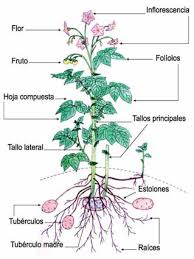
\includegraphics[scale=0.7]{planta.jpeg}
	\label{fig:planta}
\end{figure}

El desarrollo de un cultivo sigue varias etapas que son descritas en la tabla \ref{fig:cultivo} donde se observan los estados y descripción de cada etapa fenológica y la columna DDS que indica los días después de siembra.\\

\begin{figure}[h!]
	\caption{Etapas de desarrollo del cultivo de S. tuberosum Grupo Phureja variedad Criolla Latina. (Piñeros, 2009)}
	\centering
	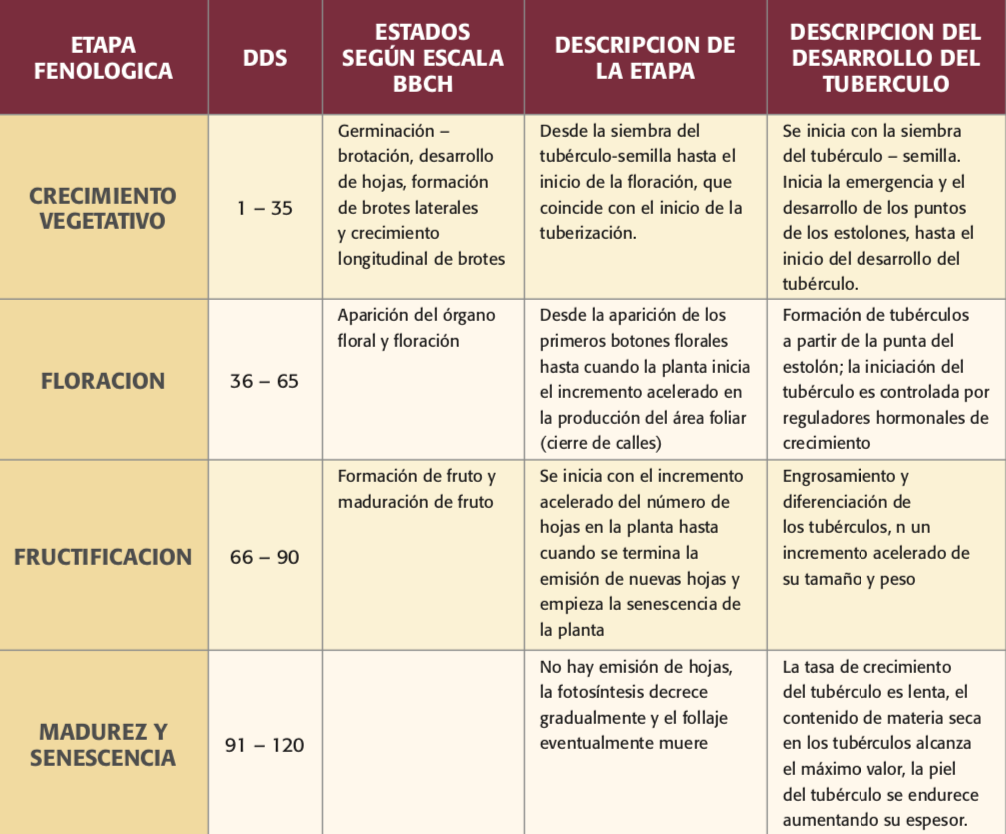
\includegraphics[scale=0.8]{papas.png}
	\label{fig:cultivo}
\end{figure}

En cuanto a su siembra los requerimientos de agua son muy importantes, los agricultores hacen coincidir esta etapa con el inicio de las lluvias o durante las mismas y emplean entre 0.6 y 0.95 toneladas de tubérculo-semilla por héctarea, la siembra suele realizarse creando surcos y calles o hileras, su disposición puede ser observada en la figura \ref{fig:surcos}.

\clearpage

\begin{figure}[h!]
	\caption{Disposición de las plantas de papa criolla en una siembra.}
	\centering
	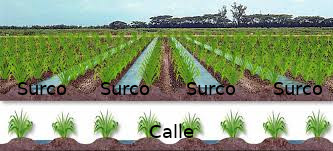
\includegraphics[scale=0.8]{surcos.jpeg}
	\label{fig:surcos}
\end{figure}

\subsection{Glosario}

\paragraph{Densidad de siembra}: Se define como el número de plantas por unidad de área de terreno.

\paragraph{Hilera}: Se define como una fila en la que son plantadas las semillas en distancias iguales.

\paragraph{Surco}: Se define como hendidura que se hace en la tierra con el arado, esta hendidura se encuentra entre cada hilera de la siembra.

\paragraph{Tubérculo}: Es un tallo subterráneo, donde se acumulan los nutrientes de reserva para la planta.



